\section{Thermal Imaging System}
In this section we describe the different components of our prototype, {\it Thermal Imaging System}. The two subsystems are the {\it Complete Camera Module} and the {\it Image Processing Unit}. We describe the configurations and the operating principles of each of the components below.

\begin{figure}[!htb]
\begin{center}
 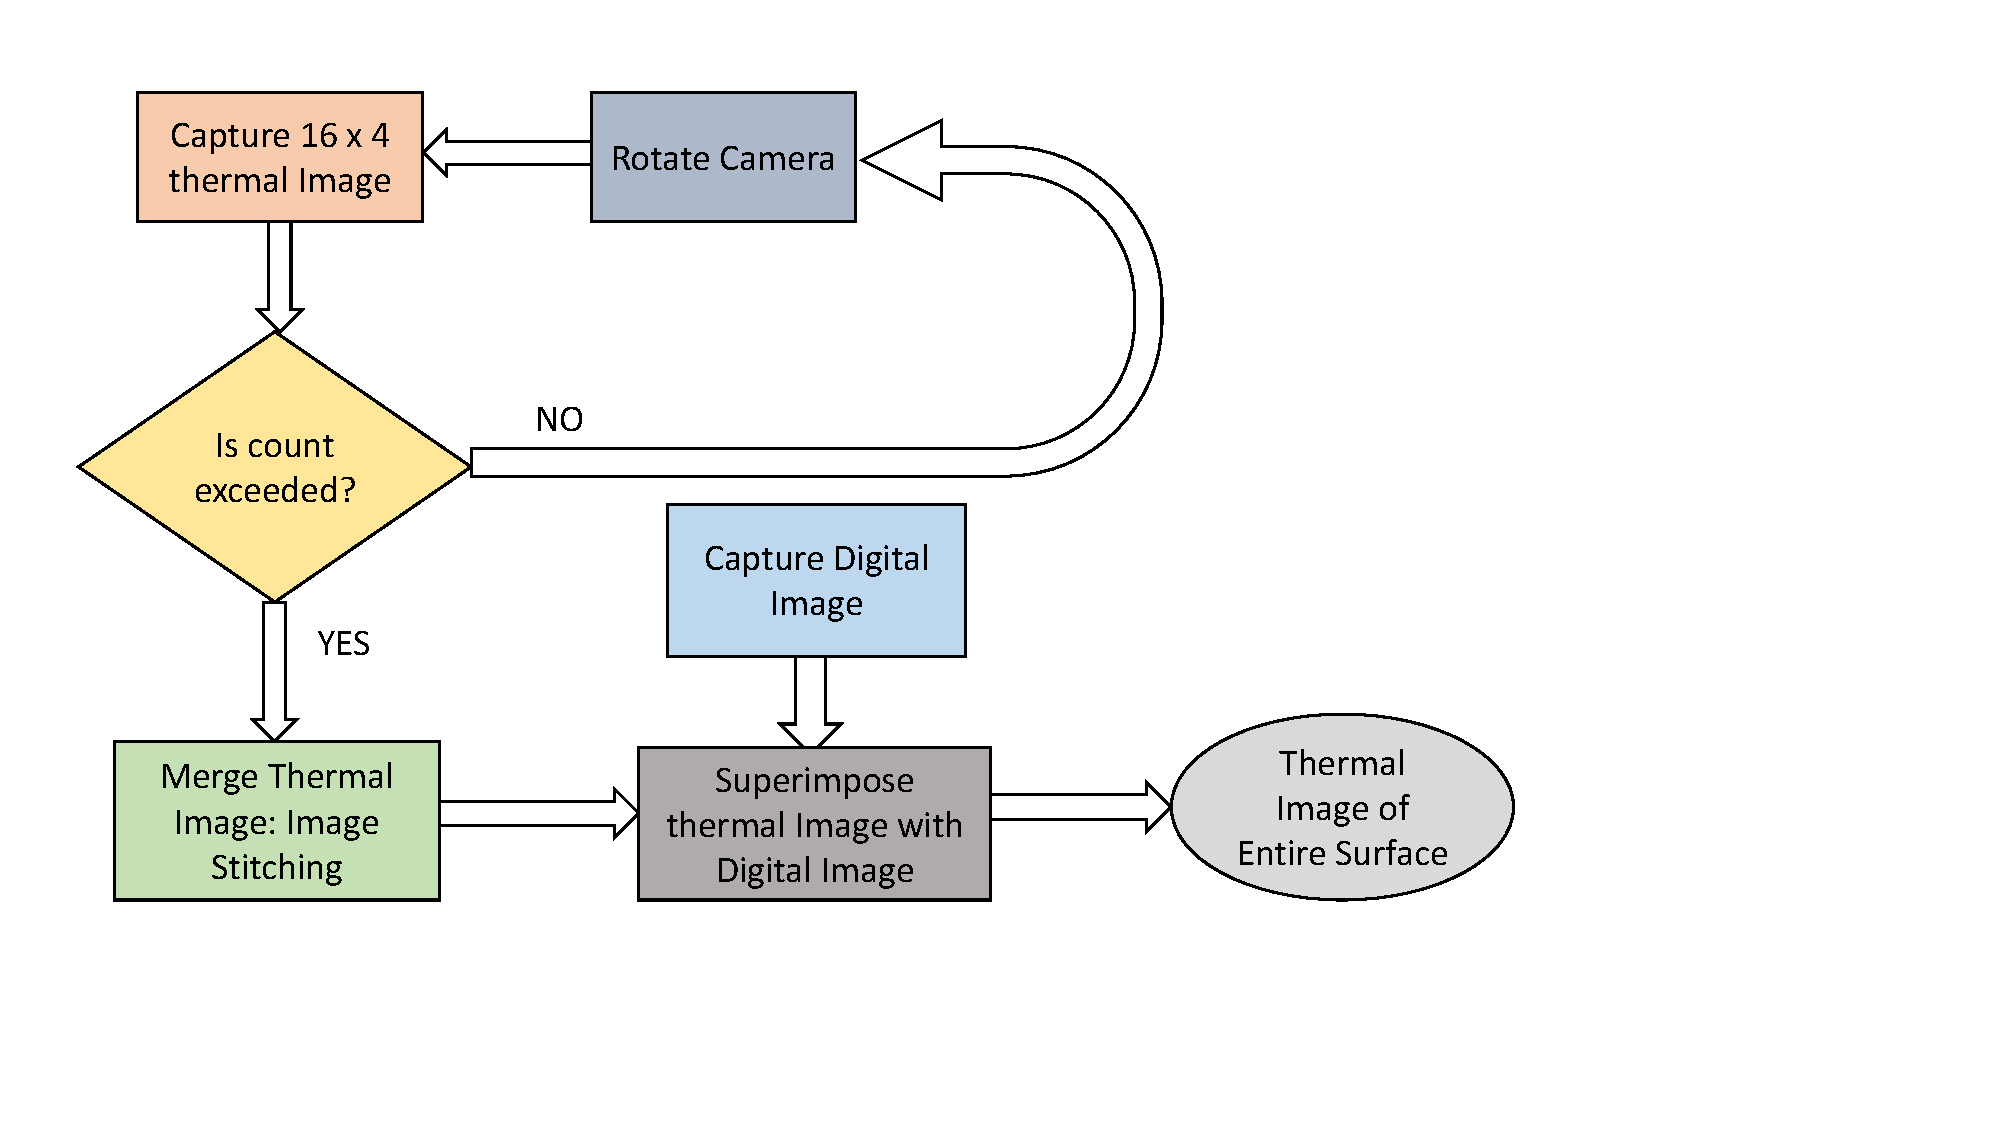
\includegraphics[width=2.8in]{figs/FlowDiagram.pdf} 
 \caption{Thermal Imaging System Flow Diagram}
 \label{fig:Flow}
\end{center}
\end{figure}
	
	
\subsection{Camera Module}
\label{sec:camera}

One of our goals in this work is to develop a low-cost IR camera based system for a one-time longitudinal heatmap scanning of an entire room which helps to find the potential air leakages, insulation problems or unattended and anomalous usage of any objects (doors and windows are open for a subtle amount of time or air leakages are quite persistent) and appliances (refrigerator door is kept open, washer is unnecessarily getting heated). While commercially available systems are available to perform the scanning but they are expensive and warrant professionals to operate. Motivated by this, we integrate a low-cost, near zero-power IR camera (MLX90621)~\cite{MLX} with a Raspberry Pi to build a simple prototype which can be deployed at ease by the home owners, residential and commercial occupants at their own comfort. 

The IR camera helps detect the background radiant temperature between -40$^{\circ}$C to +85$^{\circ}$C with a resolution of 0.02$^{\circ}$C and -50$^{\circ}$C to -300$^{\circ}$C for the object temperature and generates the corresponding heatmaps. We also integrate a digital camera with the circuit board to collect the  pictures of the scanned area for mapping the control points of the objects of interest with the heatmaps. We employ a simple image stitching algorithm to map the boundaries and contours of the objects with the heatmaps and validate them with the ground truths as obtained from the digital images. 

%Figure~\ref{} depicts the circuit for the two camera modules.
	
To achieve a 360$^{\circ}$ scanning views at a specific angle, we integrate a stepper motor unit with our proposed camera module. The entire camera module is mounted on a case which is rotated by the stepper motor. The stepper motor is calibrated to move at 5$^{\circ}$ with a low frequency to capture the thermal images. A digital camera is synchronised with the IR camera in-situ to take the images of the surrounding wall surfaces and the objects/appliances as the IR camera scan through. The data from both the IR and digital cameras is stored locally and transferred to the server periodically.
	
\subsection{Image Processing Unit}
\label{sec:imageprocessing}




%
%
%\begin{figure}[!hp]
%	\begin{minipage}{0.00\textwidth}
%		\mbox{}
%	\end{minipage}
%	\begin{minipage}{0.48\textwidth}
%		\begin{center}
%			\scriptsize{
%				\fbox{\parbox{5cm}{\texttt{
%							\begin{tabbing}
%								\=Procedure Hot and Cold Zone Segmentation(Input: \\Constructed panoramic thermal image ($I$)\\
%								\> Output: Matched Thermal Regions\\
%								1. \= Apply Otsu's thresholding\\
%								2. \> Find the contours of the hot and cold regions\\
%								3. \> Match the internal temperatures with the \\ List Of Surface Temperatures to determine state \\
%							\end{tabbing}}}}}
%							\caption{Thermal region identification algorithm}
%							\label{algo:Two Object}
%						\end{center}
%					\end{minipage}
%\end{figure}

We propose to use the IR camera in tandem with a digital camera to detect and appropriately map the heatmap's points of interest in contrast to the presence of buildings air leakages, heat dissipation associated with different objects and appliances while achieving high precision and detection accuracy. While the specific color codes of heatmaps help detect the moderate, extreme or regular hot and cold surfaces, augmenting this with digital images helps detect any unusual usage behaviors, and operating conditions of everyday appliances in smart home environment. For example, if a room has multiple windows and doors with air leakages or multiple similar small to medium load appliances, solely the heatmaps may not provide the home owners the adequate information as needed to detect any abnormal energy usage. While the IR camera albeit helps detect the region of interest but fails to provide the detailed identifications of the similar type of objects and appliances.

%We develop a basic image stitching algorithm to solve this problem. We address the image displacement problems from two differing image sources and stitch the heatmaps and digital images collectively to create a complete panorama such that it can provide meaningful feedback to the tenants for their corrective actions. First we stitch together the overlapping digital images and create a single panoramic image. Subsequently, we use the thermal images from the IR camera and stitched them together. We use the Hugin tool~\cite{XXXX} for this thermal image stitching purpose. Figure~\ref{fig:Individual} represents the individual digital image-stream as baseline. The stitched image and thermal mask are also shown in Figure~\ref{fig:Stitch}. %The fridge and the heaters are shown in the image. Our assumption is under normal conditions there is no one around and all appliances are off, so when anyone moves in or a hot or cold surface shows up then the that will show up.

We employ the digital stitching procedure to create the thermal panorama. We first stitch the digital images and maintain the respective control points for the stitching procedure which we reemploy to process the stitched thermal image generation. Next we augment the digital image in the background of the stitched thermal image based on the respective control points.% as shown in Figure~\ref{fig:Stitch} (b).
 We use a hybrid image construction methodology where the mask image or the thermal image is passed through a low pass filter and the digital image is passed through a high frequency filter to construct the digital image augmented heatmaps. A complete procedure of the this image processing step have been described in Algorithm~\ref{algo:IPU}. We then apply a image segmentation algorithm described in Algorithm~\ref{fig:Flow} to determine the different heatzone clusters in the stitched image. The temperature of each cluster is them compared with entries in a lookup table to determine the state of a specific appliance. For instance, we pre-measure the surface temperature of the refrigerator with the door open at 40$^{\circ}$F  and store it in the lookup table. If the measured temperature of the cluster is closest to 40$^{\circ}$ F then the system determines that the refrigerator door is open.

%After the digital stitch is constructed a project .pto file is created. Now if this .pto file is loaded in the tool again then it will search for the initial set of images used in the same folder. The trick is to replace these digital images with the corresponding thermal images. Although the thermal image offsets have not been aligned we get close results with thermal reconstruction. During the testing phase when an unknown set of thermal images are to be merged, we used the same .pto file for baseline digital image panorama construction for the new thermal reconstruction. When the two images are merged together the thermal mask is created for new images which identifies the open fridge or someone standing etc. One problem with the tool is during panorama construction is if someone moves the process fails. \\

%Final part consist of merging the digital panoramic image with the thermal panoramic image. The process used is hybrid image construction, where the mask image or the thermal image is passed through a low pass filter and the digital image is passed through a high frequency filter and then the two images are combined. A complete procedure of the IPU have been described in Algorithm~\ref{algo:IPU}.

\begin{figure}[!hp]
	\begin{minipage}{0.00\textwidth}
		\mbox{}
	\end{minipage}
	\begin{minipage}{0.48\textwidth}
		\begin{center}
			\scriptsize{
				\fbox{\parbox{5cm}{\texttt{
							\begin{tabbing}
								\=Procedure IPU(Input: Individual set of baseline digital \\
								\;\; images($D$) and corresponding thermal images ($I$)) \\
								\> Output: Thermal Panoramic Image\\
								1. \= Create panoramic image for the\\ 
								\;\;baseline digital images using Hugin tool\\
								2. \> Replace the digital images with the thermal images\\ 
								\;\; and load the saved project again to construct the\\ 
								\;\;panoramic thermal image\\
								3. \> Employ High pass filter on the digital image \\
								4. \> Employ Low pass filter on the IR image \\
								5. \> Combine the two to get masked thermal image
							\end{tabbing}}}}}
							\caption{IPU procedure}
							\label{algo:IPU}
						\end{center}
					\end{minipage} 
				\end{figure}